\section{Whistle Source Direction Estimation} \unsure[]{whistle-source direction esimation}
\label{subsec:03_directionEstimation}

% started with \ac{WSDE}
Considering only one stand-alone system, i.e. one robot with four microphones,
only the direction of a sound source can be
estimated.
As shortly introduced in \cref{subsec:03_whistleLocalizationStructure},
the \lstinline!WhistleDirectionEstimation! module is responsible to
determine the direction of the whistle-sound detected by the \lstinline!WhistleDetection!.
Before going into detail, the overall structure of the \ac{WSDE} on a single robot
is summarized by means of \cref{fig:04_stateMachine}.
% -------------------------------------------------------------

\begin{figure}[ht]
	\centering
		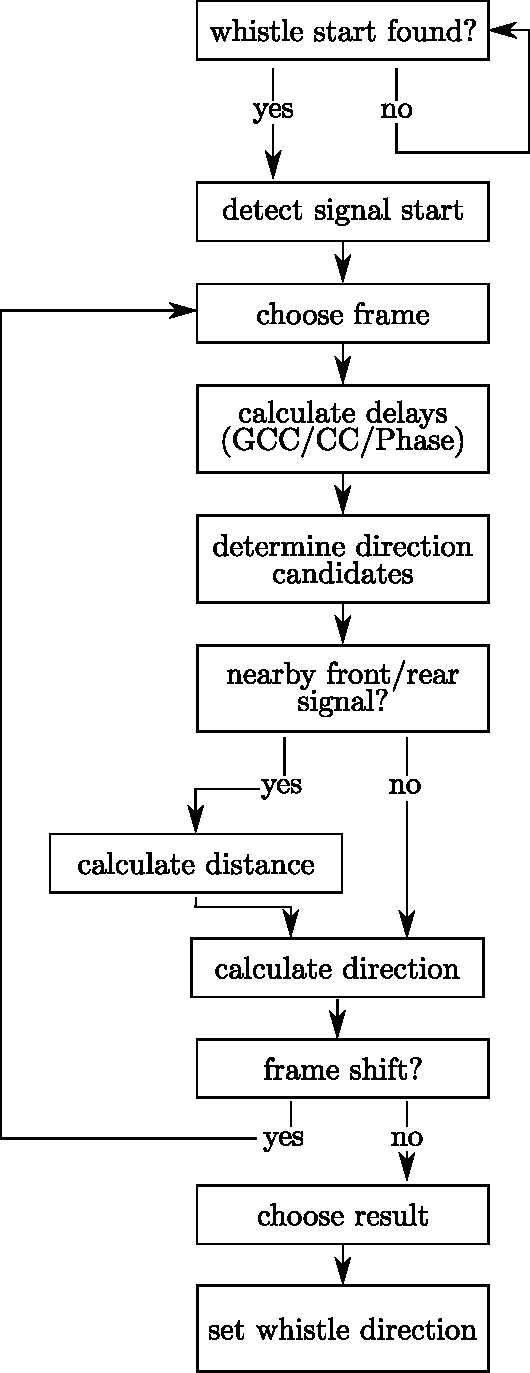
\includegraphics[height=0.7\textheight]{figures/state_machine}
	\caption{Concept of whistle localization on single robot.}
	\label{fig:04_stateMachine}
\end{figure}
% -------------------------------------------------------------

\lstinline!WhistleDirectionEstimation! depends on the data type \lstinline!WhistleData!
which is produced by the \lstinline!WhistleDetection! module and contains two values.
A timestamp when the whistle was last detected
and a boolean value if a whistle start is found.
Until this value is set to true by the \lstinline!WhistleDetection!, the
\lstinline!WhistleDirectionEstimation! buffers up to
44100 audio samples per channel.
As a whistle needs to be detected for multiple cycles in a short time, one can
be sure that the buffer contains a number of whistle samples.

Out of the buffered samples, the signal start is calculated
according to the selected signal start detection
which will be further described in \cref{subsec:03_signalStartDetection}.

Frames considered for the delay estimation
are chosen in a different way depending on the \ac{TDOA} method.
Detailed descriptions are given in the corresponding method
\cref{subsubsec:03_cc,subsubsec:03_phase}.
Using \ac{TDOA}, the delays between two microphone channels are either
determined by \ac{CC}, \ac{GCC-PHAT} or the phase difference method.
As previously stated, there exist various \ac{GCC} filter.
However, in this work by \ac{GCC} the \ac{GCC-PHAT} method is always referenced
if not explicitly specified differently.
Each delay generates two potential source direction candidates as stated
in \cref{sec:02_tdoa}.
In the event of candidates indicating a nearby signal from straight forward or
backwards, the distance to the source is estimated in addition.
More precise explanation is given in \cref{subsec:03_distance}.
For a final direction, the mean of the candidates with smallest difference
is formed.
This means that each candidate of a channel pair is compared to the other resulting candidates
of the remaining channel combinations.
The combination with the smallest sum of angular error between the candidates is selected as
\acl{WSDE}.

If one of the correlation methods is used, the \ac{TDOA} is calculated
multiple times by shifting the frame over samples.
The shift range around the start index, as well as the size of the shift, are parameterized.
By saving the calculated \ac{TDOA} values and checking certain conditions per frame shift,
the most promising \todo{etwas klarer waere hier etwas wie: best result according to the metric given in eq. XX } result can be chosen.

This way, potential start estimation inaccuracies can be corrected and
the decision process is optimized.
In case of the \ac{GCC-PHAT}, the \ac{PSNR} provides information about
the certainty of the \ac{TDOA} estimation as \cref{subsec:04_psnr} proves\todo{mit "proves" waere ich immer etwas vorsichtig. Vielleicht eher "shows" oder "as shown in"}.
A frame shift delivers \ac{TDOA} values for each channel pair and a
mean of all \acp{PSNR} from the \ac{GCC} functions.
Comparing the frame shifts, the \ac{TDOA} results with
greatest \ac{PSNR} mean value is assumed as best performing.
The same procedure is done with the \ac{CC} method but by examining
the greatest \ac{CC} function value.

Regardless of the method, the production of this module is a
\lstinline!WhistleDirection! data type which contains calculated
direction outcome in radians and additional information like distance or \ac{PSNR}.

All transformations into frequency domain and inverse transformations
are executed with the \ac{FFTW} library just as the \lstinline!WhistleDetection!.
For parallel development in Python, the widespread package \textit{NumPy} \todo{version} delivers
all fundamental functions for computation in frequency domain.

% -------------------------------------------------------------

\subsection{Signal Start Detection}
\label{subsec:03_signalStartDetection}

As mentioned in \cref{sec:02_signalStartDetection}, the detection of the
signal start is crucial for the localization.
The implementation of the different approaches will be presented coupled with
an examination of real measurement data.
To reduce undesirable effects and demonstrate the simplest form, a sinusoidal
signal of $3\si{\kilo\hertz}$ was recorded with the same circumstances as the
whistle sounds.
For the following data, the sound source was placed $2\si{m}$ in front of the robot.
In order to find the time point where the signal starts, information about
smaller fractions are required.
So, the original $44100$ samples that were buffered by the
\lstinline!WhistleLocalization! module are divided into several overlapping
frames with size $256$. The computational effort raises with smaller frame size,
but delivers a higher precision in return.
In order to perform the \ac{FFT} most efficiently, the size of one frame
should be a power of 2.
To compute the energy and entropy, the frames are transformed into
frequency domain with the \ac{FFT}.
The \ac{ZCR} does not require such a transformation.
In the evaluation \cref{sec:04_signalStartDetection}, the result of the single
methods are compared to each other.
For better visualization, the following data is shortened to $2400$ samples.

\missing[]{Start detection by frequency, whistle detection}

\subsubsection*{Spectral Entropy}

The formula to calculate the spectral entropy of a signal is introduced as
\cref{eq:02_entropy} in the previous chapter.
For the entropy information, the signal must not be cleaned previously.
By looking at the derivation of the entropy, a global minimum can be found
at the starting point of the signal due to its change from noise to signal.
The starting index is therefore defined by the index of the derivation's minimum.
Of course, this approach does not work real-time but with small delay.
\Cref{fig:03_entropy} is a plot of the recorded sine signal with the corresponding
entropy.
According to the frame size, the accuracy of the start index can be increased.
However, the frame size is limited by the required number of samples for one \ac{FFT} and
its computational effort.
% -------------------------------------------------------------
\begin{figure}[ht]
	\centering
		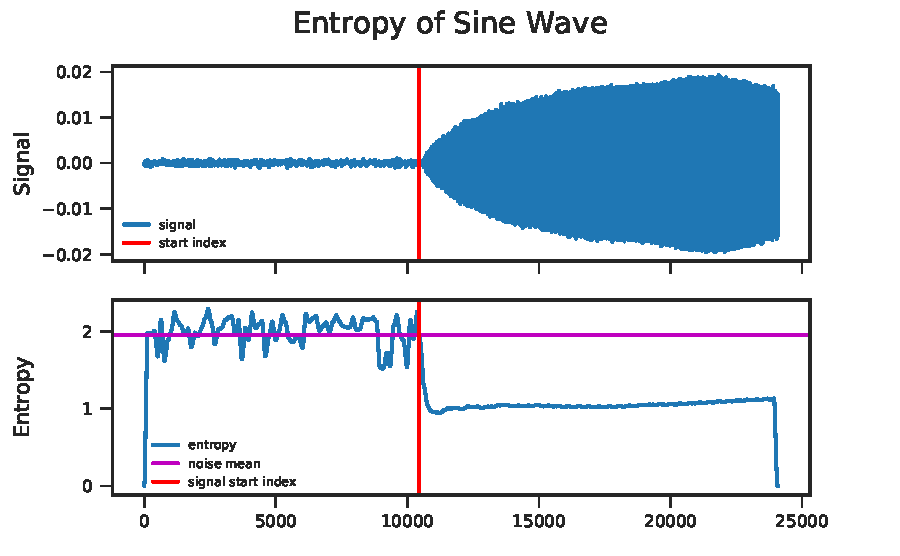
\includegraphics[]{figures/sine_entropy}
	\caption{Exemplary entropy of a sinusoidal signal with 3\si{\kilo\hertz}.}
	\label{fig:03_entropy}
\end{figure}
% -------------------------------------------------------------
In \cref{subsec:04_entropy}, the entropy outcome of a whistle sound
and its derivation is presented for evaluation.

\subsubsection*{Energy}

As mentioned above, the total signal is divided into multiple overlapping frames.
\Cref{eq:02_spectralEnergy} represents the energy of each frequency
component.
According to this, the energy of one of those frames is \cref{eq:02_energy}.
Assuming that the energy holds for the whole frame, overlapping and adding the energy
results in \cref{fig:03_energy}.
If the frequency of the examined signal is known as for the whistle, only energy values
of the relevant frequencies needs to be considered.
One downside of the energy information is that the threshold has to be adapted
manually for the related environment.
Especially at the tournament, parameters like these should be avoided and thus,
the start detection by energy is inconvenient.
% -------------------------------------------------------------
\begin{figure}[ht]
	\centering
		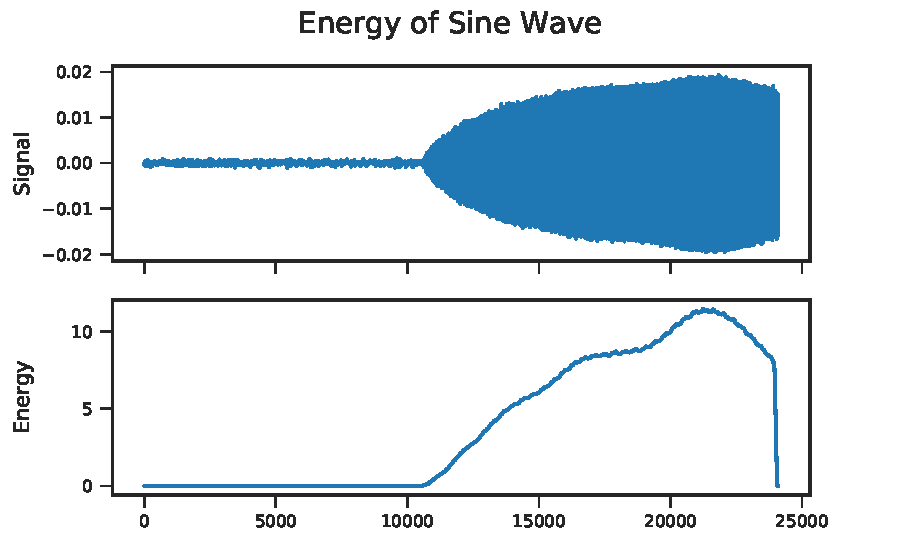
\includegraphics[]{figures/sine_energy}
	\caption{Energy of a sinusoidal signal with 3\si{\kilo\hertz}.}
	\label{fig:03_energy}
\end{figure}
% -------------------------------------------------------------

\subsubsection*{Zero Crossing Rate}

Alike the other methods, the buffered signal is divided into smaller frames
which can be set arbirary small for the \ac{ZCR} where no \ac{FFT} is necessary.
% To receive a higher accuracy, the frames of the \ac{ZCR} can be set small.
% are set to 80 samples.
In each frame, the sign changes are counted which only requires simple implementation
and computationally lightweight.
It is known that only noise is received at the beginning of the measurement and on the
contrary, signal noise is present at the end.
By comparing the mean of the received noise at the beginning of the measurement and
the mean of the signal part, a dynamic threshold can be defined and the beginning of the
signal is detectable.
In this work, the crossing of the threshold is observed from the last
value to the first.
Number of noise and signal frames are parameter values which depend
on the amount of samples and the size of the frame.
% In \cref{fig:03_zcr} and in this work, the threshold is set by multiplying the
% mean of the noise and signal mean by factor 1,25.
\begin{figure}[ht]
	\centering
		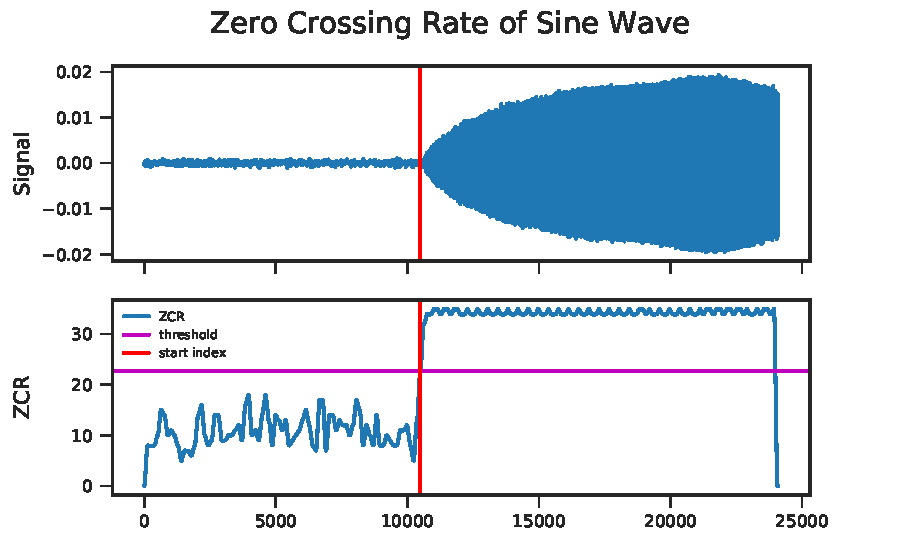
\includegraphics[]{figures/sine_zcr}
	\caption{Zero Crossing Rate of a sinusoidal signal with 3\si{\kilo\hertz}.}
	\label{fig:03_zcr}
\end{figure}
According to the circumstances, the threshold can be lowered optionally.
For real whistle data, the mean of noise and signal mean is reduced by factor 0,9 to
lower the threshold and results are shown in \cref{subsec:04_zcr}.

\subsection{Time Difference of Arrival}
\label{subsec:03_tdoa}

The \ac{TDOA} estimation is the main component to identify the
whistle source location.
Theoretical background to this approach of source localization is
given in \cref{sec:02_tdoa}.
As stated there, the \ac{TDOA} of a signal measured between two microphone sensors
provides details about the direction of the source.
Having four channels attached on a NAO's head, an overdetermined system it
given where each channel pair provides \ac{TDOA} information.

The \ac{GCC-PHAT} method is a modification of the \ac{CC} method.
Due to their implementation being equal except of the weighting function,
they are discussed in \cref{subsubsec:03_cc} collectively.
\Cref{subsubsec:03_phase} presents the implementation details with it's
circumstances.
% -------------------------------------------------------------

\subsubsection{Correlation}
\label{subsubsec:03_cc}

In theory, \acf{CC} in time domain is usually illustrated by shifting
two signals about each other and recording the similarity for each shift.
Thus, a peak will arise at that shift where signals are most similar.
Imaging two equal signals, one can image a peak at the middle of the \ac{CC} function
\lstinline!R!.
The index in this case is called \lstinline!zeroIndex! and calculated with
\lstinline!int(length(R))-1!.
If one signal is alike the other but delayed by some samples, the peak will
occur at so many samples next to the \lstinline!zeroIndex!.
This delay which is directly related to the \ac{TDOA} is computed
by the \ac{CC} and \ac{GCC} in the unit of samples.
As \cref{sec:02_cc,sec:02_gcc} have shown, the \ac{GCC} is commonly performed
in frequency domain.
For unification, both \ac{CC} and \ac{GCC} are implemented in frequency domain.
% Hereinafter, \ac{CC} and \ac{GCC} will be summarized as \textit{correlation} in this section.

The samples for the \ac{CC} are defined by the start index and the frame shift
according to \cref{subsec:03_directionEstimation} and originate from the data which was
cleaned by spectral subtraction previously.
The frame size in this work is set to 256 samples typically and the samples are Hann-windowed
prior to the correlation.
By zero padding the \ac{FFT} resolution can be increased, but is refrained from for now.
For two real signals, the \ac{CC} can be realized by time-reversing one of the signals before
the \ac{FFT} and then multiplying each component.
In the event of \ac{GCC-PHAT}, each component of the multiplication is divided by the absolute
value as the weighting function \cref{eq:02_gccPhat} defines.
After this, the cross-correlated signal is transformed back into time domain and
index of the peak \lstinline!peakIndex! is found.
The delay in samples is then computed by \lstinline!peakIndex - zeroIndex!.
In conformity with the definitions in thesis, a positive delay \lstinline!d_01!
between \lstinline!x_0! (signal at channel 0) and \lstinline!x_1! (signal at channel 1)
indicates that the signal was at channel 0 first.
% -------------------------------------------------------------

\subsubsection*{Subsample Delay}
\label{subsubsec:03_subsample}

Integer delays only offers a limited number of resulting direction angles.
To avoid this low resolution, the subsample shift estimation as in \cref{sec:02_subsampleShift}
is added to the delay estimation for both \ac{CC} and \ac{GCC}.

\subsubsection{Phase Difference}
\label{subsubsec:03_phase}

% Frame size of 64 samples -> better result
% periodicity -> maximal possible frame with given distance

In contrast to the previous methods, this method compares the phases of a
specific reference frequency per channel.
\Cref{sec:02_phase} covers the theoretical background of this approach.
The circumstances that apply on the NAOs and the appropriate implementation
is presented here.
In order to calculate the phase difference $\phi$ between two frames, the reference
frequency $f_c$ needs to be defined.
One can either choose a static reference frequency equal for all measurements or
set the reference frequency dynamically according to the sound signal.
Both implementations were realized in this work for evaluation with following
conditions:
\begin{itemize}
	\item The reference frequency must be within whistle frequency range (2\si{\kilo\hertz}
		  to 4\si{\kilo\hertz} as proposed in \cite{Hasselbring}).
	\item The maximal phase difference between two channels must not overflow $\pi$ with
		  the selected reference frequency.
\end{itemize}
Meeting this conditions, a signed phase difference is ascertainable that indicates a
distinct direction.
\Cref{tab:03_maxFrequncies} lists the maximal feasible reference frequencies (Max. Frequency)
meeting the second requirement.
As the table presents, the distance between channel 0 and 1 is too large so that the
reference frequency would need to be smaller than 2\si{\kilo\hertz}.
For this reason, the phase difference information between this pair is neglected.
% -------------------------------------------------------------
\btline{ht}{1.2}
\btab{|c|c|c|}
\hline
Channel Pairs & Absolute Distance [\si{\meter}] & Max. Frequency [\si{\hertz}]\\
\hline
0 and 1 & 0,116 & 1536,75\\
\hline
1 and 3 & 0,0533 & 3217,11\\
\hline
2 and 0 & 0,0533 & 3217,11\\
\hline
2 and 3 & 0.0618 & 2775,08\\
\hline
\etab
\et{Maximal feasible frequencies for unambiguous phase difference detection}{03_maxFrequncies}
% -------------------------------------------------------------

For compatibility with the correlation method implementation, the phase difference
is converted to delay samples $D_s$ with
\bal
	D_s = \frac{f_s \cdot \Delta \phi}{2 \pi \cdot f_c}.
\eal
% -------------------------------------------------------------

\subsubsection*{Static Reference Frequency}

Considering the sensor pair of the two front channels, the maximal feasible
reference frequency value is limited to 2775,08\si{\hertz} as stated in the table above.
Evaluation of \cref{fig:04_diffFc} has shown, that the quality of the phase difference
method relies on the reference frequency to some extent.
To realize best performance, a reference frequency between 2,6\si{\kilo\hertz} 2,775\si{\kilo\hertz}
should be chosen.
The frequency resolution of \acp{FFT} is $\frac{f_s}{N}$ depending on the sample frequency $f_s$ and
the number of data points $N$.
As the frame size for this method is set to 64 samples, the samples are zero-padded
up to 512 samples before transforming them into frequency domain for higher resolution.
With this \ac{FFT} size, it can be selected between 2670,1\si{\hertz}
and 2756,25\si{\hertz}.
Frames after the signal start index are chosen, where a whistle is detected
in all channels by the same algorithm as the existent whistle detection.
% -------------------------------------------------------------

\subsubsection*{Dynamic Reference Frequency}

In the other case, the frame is chosen by doing a frequency analysis on
multiple frames after the start index.
The frequency $f_m$ belonging to the maximal magnitude of the signal spectrum
is determined.
The first frame is chosen where $f_m$ is equal for all channels and
within whistle range.
For better understanding, the $f_m$s per frame are plotted in \cref{fig:03_maxFreq}.
Here, one sees that the conditions apply at the beginning of the whistle signal.
% -------------------------------------------------------------
\begin{figure}[ht]
	\centering
		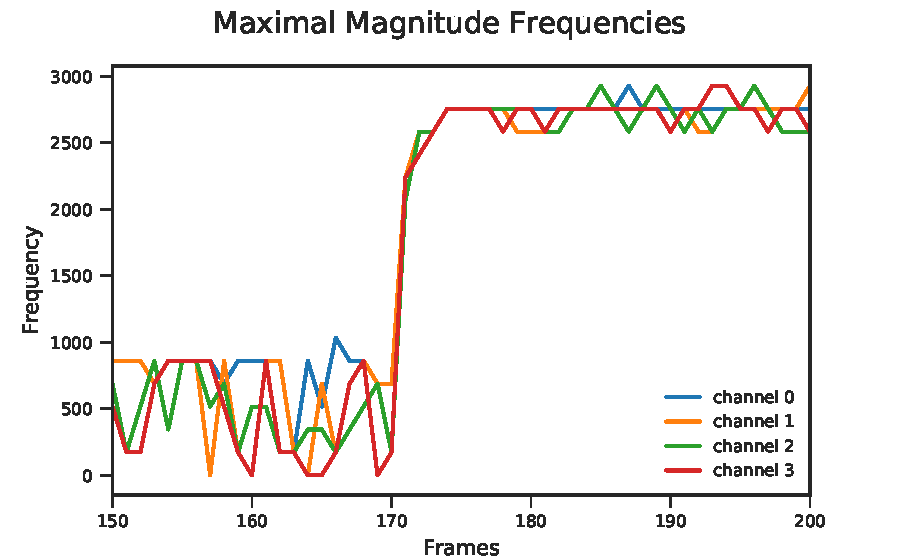
\includegraphics[]{figures/maxFreq}
	\caption{Frequencies of maximal magnitude in signal spectrum per frame.}
    \label{fig:03_maxFreq}
\end{figure}
% -------------------------------------------------------------

\subsection{Direction Estimation}
\label{subsec:03_directionCandidates}

Delay samples are computed by the \ac{TDOA} methods introduced in the last
sections.
Using \cref{eq:02_tdoaAngle}, one positive and one negative signed angle $\gamma'$
arise relative to the vector between the channels.
\Cref{fig:03_tdoaCode} is used to illustrate the terms and visualize the
circumstances for better understanding.
The definition of \textit{base channel} and \textit{next channel} stay as introduced
in \cref{subsec:03_microphones}.
Positive delay between two channels implies that a signal source
is closer to the base channel than the next channel.
For example if the detected delay has the same value as the maximum possible number
of samples between those channels, the source direction is equal to the
\textit{max-delay vector} in the figure.
In this case, $\gamma'$ is zero.
For all smaller delays greater than zero, two direction candidates \textit{candidate 0}
and \textit{candidate 1} result in the range of the max-delay vector $\pm \pi$.
The same applies mirrored for negative delays.
% -------------------------------------------------------------

\begin{figure}[ht]
	\centering
		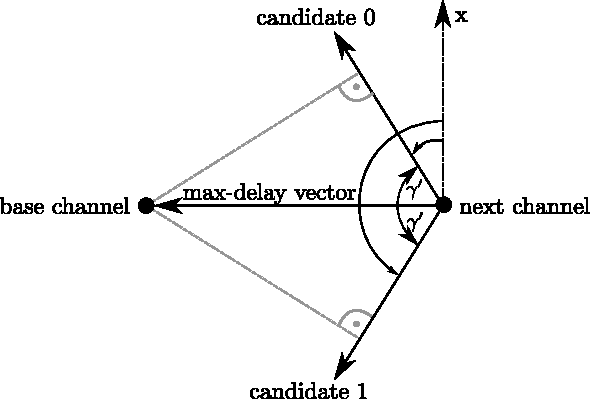
\includegraphics[width=0.6\columnwidth]{figures/tdoa_code}
	\caption{Illustration of the resulting candidates of \ac{TDOA} implementation.}
	\label{fig:03_tdoaCode}
\end{figure}

% -------------------------------------------------------------

By this implementation, all candidates are represented in the robot coordinate system.
Having four channels, each neighboring channel pair returns two candidate directions.
Diagonal channels can be paired as well for the correlation methods.
However, this case is non-observed profoundly in this work due to the overdetermined
system by four pairs.
\missing[]{Extra: evaluation of diagonal \acp{GCC}?}
Out of these eight candidates, a final direction angle $\gamma$ is chosen
by computing all combinations and selecting the one with smallest sum of angle difference.
During research, different factors like signal strength were tested to include
more a-priori knowledge.
Due to lack of reliability, no additional signal properties are taken into account.

There exists one exceptional case, where the signal source is detected straight in front
or behind the robot and distance can be estimated.
If this is the case, the direction angle is corrected to 0 or $\pi$.
How the distance information is handled is content of the next section.

\subsection{Front and Rear Distance}
\label{subsec:03_distance}

% \change[]{Image! Coordinate is not correct for set coordinate system}

% For simplicity, the direction of the sound source is determined in
% horizontal plane only.
% However, the front and rear microphones differ 0.0212\si{m} in height
% what can provide rough 
For the particular case when the signal comes straight from front or behind
the distance of the sound source can be estimated approximately.
If $delay_{01}$ (delay between channel 0 and 1) and $delay_{32}$ (delay between channel 3 and 2)
are both very small, the signal comes from
the front or the back most likely.
In theory, for this case the lateral delays are larger or equal the maximum
sample difference between the front and rear channels on the x-axis which is
to 5,41 samples.
With smaller lateral delays and some assumptions, the angle of the sound source in XZ
plane can be estimated.
\Cref{fig:02_headSideTdoa} illustrates the NAO's head from the right with
channels 1 and 3.
% -------------------------------------------------------------
\begin{figure}[ht]
	\centering
		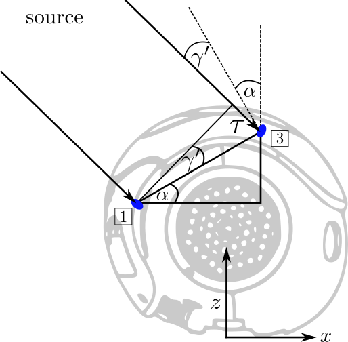
\includegraphics[width=0.45\columnwidth]{figures/side_head_tdoa}
    \caption{Illustration of arriving sound for sources from near behind.
             Adapted from \cite{nao_docu}.}
    \label{fig:02_headSideTdoa}
\end{figure}
% -------------------------------------------------------------

Assuming, that $delay_{01}$ and $delay_{32}$ are small,
the angle of the sound source $\gamma$ relative
to the Z-axis can be determined with delay $D$ as
% -------------------------------------------------------------
\bsub \bal
\gamma &= \alpha + \gamma'\\
\gamma' &= sign(D) \cdot sin^{-1}\left(\frac{D}{D_{max}}\right)\\
\intertext{whereby}
\alpha &= tan^{-1}\left(\frac{\Delta z_{channel}}{\Delta x_{channel}}\right) \approx 26,73\si{\degree}
\eal \esub
which is the angle to the orthogonal axis to the plane though
front and rear channels.
$\Delta z_{channel}$ and $\Delta x_{channel}$ are the distances between the channels
in z- and x-direction in \si{\meter}.
% -------------------------------------------------------------
\begin{figure}[ht]
	\centering
		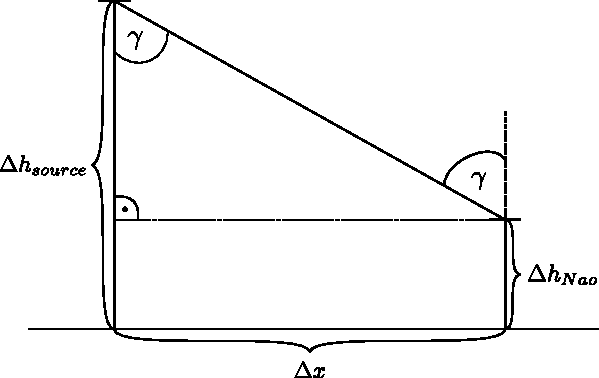
\includegraphics[width=0.6\columnwidth]{figures/x_distance}
	\caption{Illustration of distance estimation.}
    \label{fig:02_xDistance}
\end{figure}
% -------------------------------------------------------------

Known that the sound source is ordinarily positioned above of the robot, the distance
of the sound source can be approximated with an assumed height $\Delta h_{source}$
of the source. $\Delta h_{source}$ differs from referee and thus, is only
a averaged value.
So, the distance in x-direction $\Delta x$ is
% -------------------------------------------------------------
\bal
\Delta x &= (\Delta h_{source} - \Delta h_{NAO}) \cdot \tan(\gamma).
\label{eq:02_deltaX}
\eal
% -------------------------------------------------------------

The distance estimation is triggered, if the direction candidates of
$delay_{01}$ and $delay_{32}$ are smaller than $\pm$ 10\si{\degree}
or larger than $\pm$ 170\si{\degree}.
Additionally, the lateral delays must be smaller than 5,41 samples as mentioned above.

Restrictions of the front and rear distance measurement differ.
For the front case, the maximum angle for a unambiguous distance calculation
is $\frac{\pi}{2}- 2\alpha$.
Thus, the maximum front distance that can be approximated shrinks to
$\Delta x = (\Delta h_{source} - \Delta h_{NAO}) \cdot \tan(\frac{\pi}{2} - 2\alpha)$
according to \cref{eq:02_deltaX}.
To the rear, the maximum value for $\gamma$ is bounded by the 5,41 samples that
are set as condition.
Setting $\Delta h_{source}$ to 1,5\si{m} and $\Delta h_{NAO}$ to 0,57\si{\meter} for example,
the maximum measurable distance to the front is about 0,66\si{\meter}.
With the same values the maximum distance backwards is more than 50\si{\meter} in theory.
However, measurements in \cref{subsec:04_distance} show that 7\si{\meter} is the
limit for the real case.

% -------------------------------------------------------------

\subsection{SNR}
\label{subsec:03_snr}

The \acf{SNR} is a common value to express the signal power $P_{signal}$ compared
to power of the background noise $P_{noise}$.
Conveniently, the buffered audio signal in this thesis always consists of
a clean-cut delimitation between signal and noise which is set by the
start index.
Thus, the \ac{SNR} which is defined as
\bal
    SNR_{db} = 10\log_{10}\left(\frac{P_{signal} - P_{noise}}{P_{noise}}\right)
    \label{eq:03_snr}
\eal
in decibels can be implemented straightforwardly.
Informational content about this measure is investigated in \cref{subsec:04_snr}.
Expectations are that the \ac{SNR} can be feed into the covariance matrix
of an incoming result in the Bayesian update process.

\subsection{PSNR}
\label{subsec:03_psnr}
In image processing, the \acf{PSNR} indicates the quality of a compressed
image. Here in this work, the ratio between the peak of a signal
and its noise is related to the \ac{GCC-PHAT} outcome and called \ac{PSNR}
henceforth.
As stated in \cref{sec:02_gcc}, the most significant characteristic
of the \ac{GCC-PHAT} is the resulting sharp peak which now can be
assessed with one value
\bal
    PSNR_{db} = 10\log_{10}\left(\frac{P_{peak}}{P_{noise}}\right).
    \label{eq:03_psnr}
\eal
From the implementation view, the power of the correlation peak is divided by
the power of the remaining correlation signal.
It has to be noted that two adjacent values prior and after the peak
are disregarded as they might belong to the peak.
A validation if and how much the \ac{PSNR} and the accuracy of the \ac{GCC}
delay result are linked is done in \cref{subsec:04_psnr}.
% -------------------------------------------------------------